\chapter{Sound Source Localization \& \library{Mirage}}\label{chap:mirage}

\marginpar{%
    \footnotesize
    \textbf{Keywords:} Sound Source Localization, Image Microphones, Acoustic Echoes, TDOA Estimation.
    \\\textbf{Resources:}
    \begin{itemize}
        \item \href{https://ieeexplore.ieee.org/document/8683534}{Paper}
        \item \href{https://github.com/Chutlhu/mirage}{Code}
        \item \href{https://sigport.org/documents/mirage-2d-sound-source-localization-using-microphone-pair-augmentation-echoes}{Poster}
    \end{itemize}
}

\newthought{Synopsis} \synopsisChMirage

\mynewline
Together with~\cref{ch:lantern}, this chapter describes methods and results published in~\cite{di2019mirage}, which considers only stereophonic recordings.
In this sense, this chapter provides an application of the~\cref{ch:lantern}.
Subsequently, the proposed approach was to multi-microphone recordings in collaboration with Randy Gomez from Honda Research Institute.


% \subsection{Literature review: an acoustic perspective}
% Bibliography with respect to sound propagation

% \subsection{Literature review an algorithmic perspective}
% Bibliography with respect to learning and knowledge approaches

% \newthoughtpar{Knowledge-based vs. learning-based approaches}

% \newthoughtpar{Regression vs. classification approaches}

% \section{Background in SSL}
% \begin{itemize}
%     \item 1D SSL: AOA estimation
%     \item 2D SSL: azimuth and elevation estimation
%     \item 3D SSL: polar and cartesian coordinates
% \end{itemize}

% \subsection{Stereophonic SSL and 1D SSL}

% \newthoughtpar{Binaural SSL}

% \subsection{Multichannel SSL and 2D SSL}

% \section{\mirage: microphone augmentation with echoes}

% \section{Experimental evaluation}

% --- Margin Figure
\section{Literature review in Echo-aware Sound Source Localization}
Common to most sound source localization approaches reviewed in ~\cref{subsec:application:localization} is the challenge posed by environment reverberation.
It is typical to observe that \ac{DOAs} estimation degrades with increasing acoustic reflection~\citeonly{chen2006time}.
For these reasons, most sound source localization methods regard reverberation and, in particular, acoustic echoes as a nuisance.
Room reverberation is considered in the works~\citeonly{rui2004time, chen2006time, zhang2007maximum} while the authors of~\citeonly{weinstein1994iterative, taghizadeh2015spatial, salvati2016sound} attempt to solve \SSL/ by estimating the full \RIRs/.
However, both the cases have drawbacks: in the former, the generic model for reverberation does not reduce strong early echoes, and in the latter, \RIRs/ estimation is a difficult task.

\mynewline
The echo-aware sound source localization methods take another direction: they exploit the closed-form relation between echoes timings and audio scene geometry expressed by the \ISMdef/.
Early works such as~\citeonly{korhonen2008acoustic, ribeiro2010turning, ribeiro2010using, svaizer2011use} uses knowledge form the room geometry to estimated the position of the sound source with respect to the arrays.
This idea was subsequently extended in later works, reducing the amount of prior knowledge required or addressing different applications.
The authors of \citeonly{nakashima2010localization}  study the \SSL/ problem in binaural recordings.
To improve localization, they propose to used ad-hoc reflectors as artificial \textit{pinnae} and a simple reflection model.
In the work~\citeonly{krekovic2016echoslam}, the author addresses the problem \ac{SLAM}\sidenote{
    \ac{SLAM} enables the estimation of a moving robot’s position in relation to a number of external acoustic sources.
} using echoes.
The authors of~\citeonly{an2018reflection} propose to use cameras, depth sensors, and laser sensors to identify reflectors and build a corresponding acoustic model that is used
for echo-aware \ac{SSL}.
Finally, in a very recent work, the well-known \ac{MUSIC} framework for localizing multiple sources is modified for accounting an echo model for the spherical harmonic representation~\citeonly{birnie2020reflection}

\mynewline
All the above mentioned echo-aware methods are explicitly knowledge-driven, namely, using closed-form solutions based on physics, acoustics, and signal processing models.
As explained in the previous chapter, data-driven methods, especially \ac{DNN}, have been successfully applied to address \SSL/.
The main benefit is in their ability to learn complex mapping functions based on simple input-output pairs.
However, they are typically trained for specific applications and use-cases (\eg/, arrays geometry, acoustic conditions, \etc/) and fail whenever test conditions strongly mismatch training conditions.

\section{Proposed Approach}
In the work \cite{di2019mirage} we proposed to combine the best of the two worlds:
using a deep learning model to estimate challenging acoustic parameters and a physically-motivated model to map such parameters to source's \DOAs/.
To this end, we introduce the framework of \MIRAGEdef/ for \SSL/, based on the \textit{image microphones} model~\citeonly{bergamo2004collaborative,korhonen2008acoustic} (See~\cref{sec:separake:sota}).

\mynewline
Let us consider a simple yet common scenario to illustrate this idea:
two microphones, one source, and a nearby reflective surface, as illustrated in Fig. \cref{fig:mirage:scene}.
\marginpar{%
    \centering
    \footnotesize
    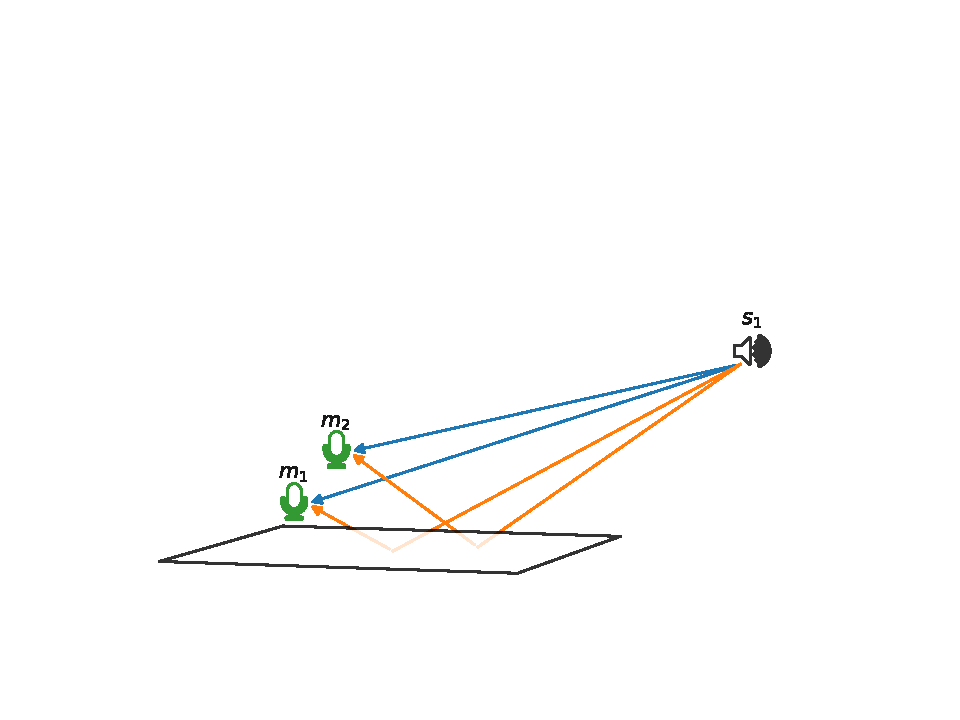
\includegraphics[trim={50 70 50 150},clip,width=\linewidth]{mirage/scene.pdf}
    \captionof{figure}{%
        Typical setup with one source source recorded by two microphones.
        The illustration shows direct sound path (blue lines) and resulting first-order echoes (orange lines).}
    \label{fig:mirage:scene}
}
This may occur when the sensors are placed on a table or next to a wall. Striking examples of these scenarios are the smart table-top devices, such as Amazon Echo, Google Home, \etc/.
The reflective surface is assumed to be the most reflective and closest one to the microphones in the environment, generating the strongest and earliest echo in each microphone.
Under this \textit{close-surface} model, we ask the following question:
\begin{enumerate}
    \item Can early echoes be estimated from two-microphone recordings of an unknown source?
    \item Can early echoes be used to estimate both the azimuth and elevation angles of the source, an \textit{impossible} task in free field conditions?
\end{enumerate}

\newthought{The First Question} was already addressed in~\Cref{ch:lantern}.
In particular, we proposed to use a \ac{DNN} trained on a simulated close-surface dataset to estimate early echoes properties from audio features.

\newthought{To answer the Second Question}, we propose the \ac{MIRAGE} framework.
It exploits echoes' time of arrival by expressing them as \acp{TDOA} in the \textit{virtual 4-microphone array} formed by the true microphone pair and its image with respect to the reflective surface.
We show that this framework approximately estimates echo properties, perform similarly to a correlation-based method in azimuth estimation for the considered
scenario and estimates \textit{impossible} elevation angles with good accuracy in noiseless settings using two microphones only.


\section{Background in microphone array SSL}\label{sec:background}
In this section, we briefly review some necessary background in microphone array \ac{SSL}.
Let us assume a microphone array of $\idxMic$ sensors is placed inside a room and records the sound emitted by one static point sound source ($\numSrcs=1$).
In all generality, the relationship between the signal $\mic_\idxMic$ recorded by the $\idxMic$-th sensor placed at fixed position $\positionMicrophone_\idxMic$ and the signal $\src$ emitted by the source at fixed position $\positionSource$ is defined by:
\begin{equation}\label{eq:mirage:anymic_time}
\mic_i[n] = (\flt_\idxMic \convDis \src)[n]  \; + \; \nse_\idxMic[n],
\end{equation}
where the convolution with \RIR/ $\flt_\idxMic[n]$ embodies the fact that sensor $\idxMic$ receives a spatial image of the source and $\nse_\idxMic$ denotes possible measurement noise.
As fully described in~\cref{ch:acoustic}, the \RIR/ depends on the spatial parameters of the scene: microphone positions, source position \wrt/ the room, as well as the room acoustic properties (size, absorption, and diffuseness of the wall materials).

\mynewline
Let us assume that \RIRs/ follows the echo model under the narrowband approximation presented in~\cref{subsec:processing:stft}.
Therefore, in the discrete-frequency domain, this leads to
\begin{equation}\label{eq:mirage:rir}
    \FLT_\idxMic[k] = \sum_{\idxEch=0}^{\numEchs}  \; \alpha_\idxMic^{(\idxEch)}[k] \; \cste^{- \csti 2 \pi f_k \tau_\idxMic^{(\idxEch)}} \; + \; \varepsilon_\idxMic[k],
\end{equation}
where $f_k$ is the $k$-th frequency bin and the error term $\varepsilon_i[k]$ collects later echoes, the reverberation tail, diffusion, and noise.
A time-domain example of \RIR/ is shown in Fig.~\cref{fig:mirage:rirs} (left).
In this work, we will consider only the first strongest echo, therefore $R = 1$.
Note that $r=0$ denotes the ideal propagation path.

\begin{figure}[t]
    \begin{sidecaption}[RIRs within the MIRAGE framework]{%
        (Left) A typical simulated \RIR/ with annotated components.
        (Right) Superposition of two RIRs and visualization of time difference
        of arrival between direct paths (\ac{TDOA}), first echoes (\ac{iTDOA}) and direct path and first echo (\ac{TDOE}).
    }[fig:mirage:rirs]
    \centering
    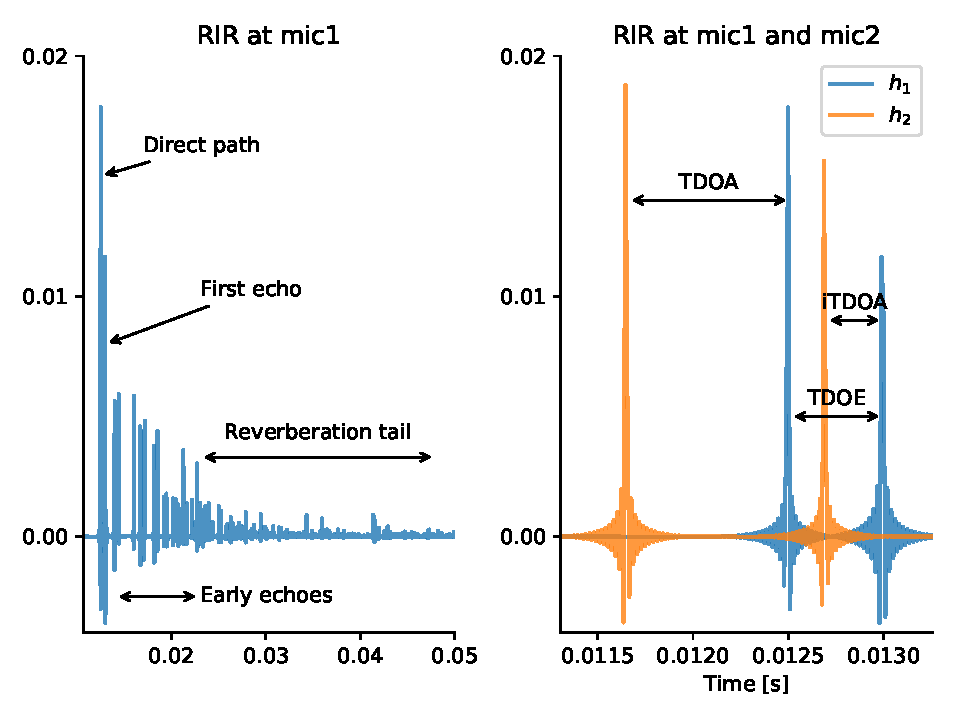
\includegraphics[trim={0 0 0 0},clip,width=\linewidth]{mirage/rirs.pdf}
    \end{sidecaption}
\end{figure}


\subsection{2-channel 1D-SSL}\label{subsec:mirage:1D-SSL}
\newcommand{\tdoa}{\ensuremath{\tau_\mathtt{TDOA}}}
\newcommand{\aoa}{\ensuremath{\vartheta}}
Let us first consider the case of stereophonic recordings ($\numMics=2$).
Under the far-field assumption, traditional \SSL/ methods use the \acf{TDOA},
\begin{equation*}
    \tdoa \eqdef \tau^{(0)}_2 - \tau^{(0)}_1\quad\text{[second]}
    ,
\end{equation*}
as a proxy for the estimation of the \ac{AOA}, $\aoa$, since:
\begin{equation}\label{eq:mirage:aoa}
    \vartheta = \arccos \kparen{\speedOfSound \: \tdoa \: / \: \distMicMic }\quad\text{[rad]},
\end{equation}
where $\speedOfSound$ is the speed of sound and $\distMicMic$ the inter-microphone distance.

\mynewline
Then, \SSL/ reduces to estimating the \ac{TDOA}, which can be done by cross-correlation-based methods such as the widely used and well performing \ac{GCC-PHAT} method \citeonly{knapp1976generalized, blandin2012multi}.
Given \STFT/ $\MIC_1$ and $\MIC_2$ of the two microphones signals, the \ac{GCC-PHAT} \textit{angular spectrum} is defined as:
\begin{equation}\label{eq:mirage:gccphatcontrast}
\Psi_\mathtt{GCC}(\tau) = \sum_{k,l}\frac{\MIC_1[k,l] \khermitian{\MIC}_2[k,l]}{\kvbar{ \MIC_1[k,l] \khermitian{\MIC}_2[k,l] }} \cste^{-\csti 2  \pi f_k \tau}
,
\end{equation}
where $\kvbar{\cdot}$ denotes the absolute value.

\mynewline
Then, the \ac{TDOA} estimate is given by
\begin{equation*}
    \hat{\tau}_\mathtt{TDOA} = \arg \underset{\tau}{\max} \; \Psi_\mathtt{GCC}(\tau)
    .
\end{equation*}
Note that $\Psi_\mathtt{GCC}$ can also be expressed directly as a function of the \ac{AOA} using \eqref{eq:mirage:aoa}, hence the term \textit{angular spectrum}.
Despite the theoretical limits of this method, discussed in~\citeonly{chen2006time}, this method is known to work well in practice.
Moreover, it was showed to be state-of-the-art for \ac{SSL} in a large benchmark study~\citeonly{blandin2012multi}.

\subsection{Multichannel 2D-SSL}\label{subsec:mirage:2D-SSL}
When more microphones are available and the microphones array is compact and not linear\sidenote{
    In case of complanarity, the angle can be estimated up to ``up-down'' umbigity.
}, 2D-\ac{SSL} can be envisioned
A possible approach is to use 1D-\ac{SSL} on all pairs and combine their results, a principle which was successfully applied in the \acf{SRP-PHAT} method \citeonly{dibiase2001robust}.

\begin{figure}
    \begin{sidecaption}[]{
        Illustration of the relation between \ac{DOA} and \ac{TDOA} with ones source and two microphone.
        Knowing the distance $\distMicMic$ between the two microphones, simple trigonometry yields the \ac{AOA} $\vartheta$ according to~\cref{eq:mirage:aoa}.
    }[fig:mirage:gcc]
        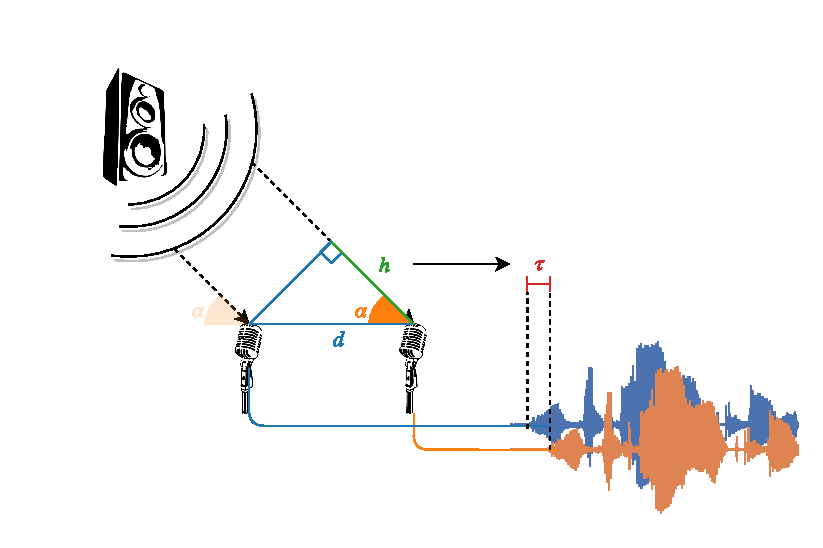
\includegraphics[width=\linewidth]{mirage/tdoa_microphone.pdf}
    \end{sidecaption}
\end{figure}

\mynewline
The \ac{SRP-PHAT} methods returns the source's \ac{DOA}, namely the pair azimuth and elevation $(\theta, \phi)$, by estimating \acp{TDOA} from each microphone pairs.
In order to achieve this, it requires the geometry of the microphone array to be known.
In a nutshell, this algorithm aims to estimate a \textit{global angular spectrum} $\Psi_{\mathtt{SRP}}(\theta,\phi)$ in the polar coordinates system with respect to reference point in the array, typically its barycenter.
This function will exhibit a local maximum in the direction of the active source.
\\The algorithmic can be exemplified in the following steps:\marginpar{
    \footnotesize\itshape
    See \href{http://bass-db.gforge.inria.fr/bss_locate/}{\library{MBSSLocate}\ExternalLink} for a free MATLAB implementation and comprehensive documentation of this algorithm.
}
\begin{enumerate}
    \item a global grid of \acp{DOA} candidates is defined according to a desired resolution and computational load;
    \item for each pair of microphones, a local set of \ac{AOA} (hence, \acp{TDOA}) is defined based on the above chosen \acp{DOA} and the input geometry;
    \item a TDOA-based algorithm (\eg/ \ac{GCC-PHAT}) is used to compute the associated local angular spectrum;
    \item all the local contributions (a collection of local $\Psi_\mathtt{GCC}(\tau)$) are geometrical aggregated and interpolated back to the global \ac{DOA} grid to form $\Psi_{\mathtt{SRP}}(\theta,\phi)$;
    \item the \acs{DOA}(s) maximizing $\Psi_\mathtt{SRP}$ is (are) used as estimate (in case of multiple sources).
\end{enumerate}
This algorithm can be seen as an application of the divide-and-conquer paradigm to \ac{TDOA}-based methods:
``at the leaves'', the \ac{GCC-PHAT} method provide \ac{TDOA} for each microphone pair;
the ``merge'' operation consists in aggregating \ac{TDOA} defined on a different axis based on the knowledge of the array geometry.
Finally, we stress that this algorithm is independent of the method used to estimate the \ac{TDOA}.

\begin{figure}
    \begin{sidecaption}[]{
        Illustration of the different \acp{DOA} at each microphone pairs listening one sound source.
        Knowing the position of the microphone, the angle with respect to a reference point can be deduced in closed-form.
    }[fig:mirage:gcc]
        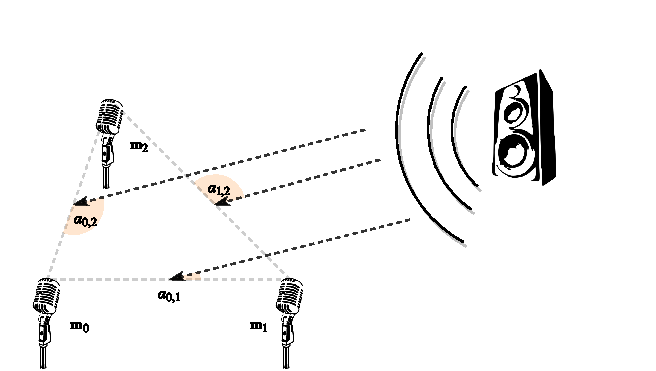
\includegraphics[width=\linewidth]{mirage/srp-phat_aggregation.pdf}
    \end{sidecaption}
\end{figure}


\section{MIRAGE: Microphone Array Augmentation with Echoes}\label{sec:mirage:mirage}
We now introduce the proposed concept of \underline{mi}crophone a\underline{r}ray
\underline{a}u\underline{g}mentation with \underline{e}choes (MIRAGE).
Let us first expand formula~\eqref{eq:mirage:rir} to account for more echoes:
\begin{equation}
\label{eq:mirage:echo_h}
H_i(f) = \sum_{k=0}^{K}\alpha_i^k(f) \; e^{- 2 \pi f \tau_i^k} \; + \; \varepsilon_i(f)
\end{equation}
where the sum now comprises the direct path ($k=0$) and the $K$ earliest reflections ($K = 1$ in this paper)
and $\varepsilon_i$ collects the remaining RIR components.
Here, $\alpha_i^k(f)$ accounts for both air attenuation and wall absorption phenomena.
In the remainder of this paper, we make the approximation of frequency-independent $\alpha_i^k$.
Eq.~\cref{eq:mirage:echo_h} then corresponds to the well known image-source (IS) model,
where reflections are treated as mirror images of the true source with respect to reflective surfaces,
emitting the same signal.
\marginpar{%
\centering
\footnotesize
    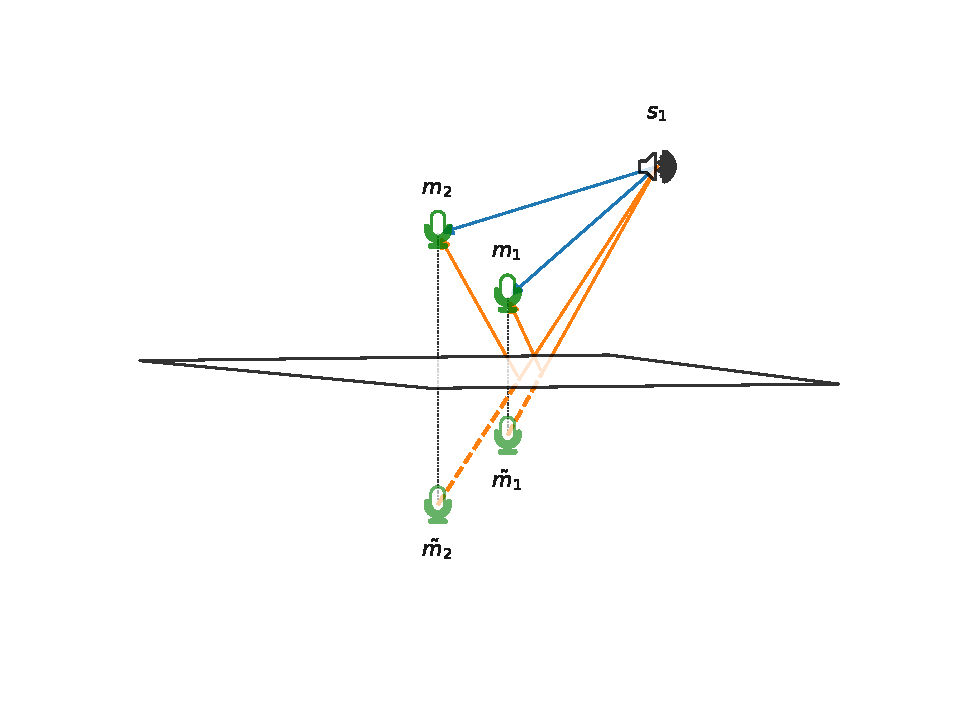
\includegraphics[trim={90 75 40 50},clip,width=\linewidth]{mirage/mirage.pdf}
    \captionof{figure}{%
        Illustration of the images $\tilde{m}_1$ and $\tilde{m}_2$ of microphones $m_1$ and $m_2$ in the presence of a reflective surface and a source.
        Blue lines correspond to direct paths, orange lines correspond to echo paths.}
    \label{fig:mirage:mirage}
}
We will employ here a less common but equivalent interpretation of IS,
namely, the image-microphone (IM) model. As illustrated in Fig.~\cref{fig:mirage:mirage},
virtual microphones are mirror images of the true microphones with respect to reflective surfaces.
In this view, the echoic signal received at a true microphone
is the sum of the anechoic signals received at this microphone and its images.
If we consider the virtual array consisting of both true and image microphones,
multiple microphone pairs are now available. For each of them,
it is then possible to define a corresponding time difference of arrival.
Among them, we will refer to the one between the two real microphones as TDOA,
the one between the two image microphones as image TDOA (iTDOA) and the one between
the first microphone and its image as time difference of echoes (TDOE).
We have:

\begin{align}
\tau_\mathtt{TDOA}  &= \tfrac{1}{c} \norm{\positionMicrophone_2 - \positionSource} - \tfrac{1}{c} \norm{\positionMicrophone_1 - \positionSource} = \tau_2^0 - \tau_1^0,\\
\tau_\mathtt{iTDOA} &= \tfrac{1}{c} \norm{\tilde{\positionMicrophone}_2 - \positionSource} - \tfrac{1}{c} \norm{\tilde{\positionMicrophone}_1 - \positionSource} = \tau_2^1 - \tau_1^1,\\
\tau_\mathtt{TDOE}  &= \tfrac{1}{c} \norm{\tilde{\positionMicrophone}_1 - \positionSource} - \tfrac{1}{c} \norm{\positionMicrophone_1 - \positionSource} = \tau_1^1 - \tau_1^0,
\end{align}
where $\tilde{\positionMicrophone}_i$ denotes the position of the image of $\positionMicrophone_i$ with respect to the reflector.
These three quantities are directly connected to \RIRs/, as illustrated in Fig.~\cref{fig:mirage:rirs}(right).

Let $V = \{ \mathtt{TDOA}, \mathtt{iTDOA}, \mathtt{TDOE}\}\in\mathbb{R}^3$.
Following the 2D-SSL scheme described in Sec. \cref{subsec:mirage:2D-SSL} and
given the virtual microphone-array geometry (which depends on the relative position of microphones to the surface),
$V$ could in principle be used to estimate the 2D directional of arrival of the source.
In the next section, we present a learning-based method to estimate
$V$ using audio features obtained from only two microphones.

% \section{Learning-based echo estimation}
% Our approach is to train a deep neural network (DNN) on a dataset simulating the considered close-surface scenario.
% We model the problem as multi-target regression, with \textit{interaural level difference} (ILD)
% and \textit{interaural phase difference} (IPD) as input features, and $V \in \mathbb{R}^3$ as output parameters.
% ILD and IPD features are defined in the frequency domain as follows:
% \begin{equation}
% \label{eq:mirage:features}
% \begin{cases}
% ILD(f)  =& \tfrac{1}{T} \sum_{t=1}^T \log{\mid \frac{M_2(f,t)}{M_1(f,t)} \mid } \\
% IPD(f)  =& \tfrac{1}{T} \sum_{t=1}^T \frac{M_2(f,t)/ \mid M_2(f,t) \mid }{M_2(f,t) / \mid M_1(f,t)  \mid}\\
% \end{cases}
% \end{equation}
% More precisely, the input of the network is
% $\mathbf{x} = [ILD,$ $\operatorname{Re}(IPD)], \operatorname{Im}(IPD)]$, where $\operatorname{Re}$
% and $\operatorname{Im}$ denote real and imaginary part operators, respectively.
% Note that for the IPD, the frequency $f=0$ is discarded because it is constant for every observation.
% In general, the mapping between $V$ and the proposed feature is not unique.
% In particular, this happen when $\tau_2^1 = \tau_1^1$.
% In order to avoid this, we preventively pruned all the entries
% with $| \tau_2^1 - \tau_1^1 | < 10^{-6}$ from the dataset.

% %The performances of cross-correlation methods (e.g. GCC-PHAT) depends on the extraction on local maxima. However in an reverberant scenario many local extrema at periodic intervals can be observed due to the reflections. So which peaks corresponds to the desired TDOA, iTDOA and TDOE? To avid this ambiguity advance methods can actually retrieve TDOAs and iTDOAs however it is challenging for them to estimate TDOE, which is an essential variable for defining an MIRAGE setup~\cref{fig:correlation}.
% %The network is a simple multi-layers neural network (DNN). It has $D$ inputs corresponding to the dimension of the input feature vector $\mathbf{x}$ and $L = 3$ output nodes corresponding to the three target variables of $V$.
% We use a simple fully-connected DNN architecture consisting of a $D$-dimensional input layer,
% a $3$-dimensional output layer, and 3 fully connected hidden layers with respective input
% sizes $500$, $300$ and $50$. Rectified linear unit (ReLU)
% activation functions are used except at the output layer,
% and each hidden layer has a dropout probability $p_\text{do} = 0.3$.
% We use the mean square error loss function for training and the Adam optimizer \citeonly{kingma2014adam}.
% The normalized root mean square error (nRMSE) is taken as validation
% metric\footnote{The nRMSE takes values between $0$ (perfect fit) and $\infty$ (bad fit).
% If it is equal to $1$, then the prediction is no better than a constant.}.
% The network is manually tuned on a validation set to find the best combination of number of hidden layers, their sizes and $p_\text{do}$.
% Once time delay estimates $\hat{V}$ are returned by the DNN, they are converted to synthetic
% local angular spectra and passed to $\Psi_\text{SRP}$ (See Sec. \cref{subsec:mirage:2D-SSL})
% together with the relative positions of true and image microphones which are assumed known.
% We call this algorithm MIRAGE. The synthetic local angular spectra consist of Gaussians
% centered at $\hat{V}$ and with variances equal to the prediction errors made by
% the DNN on the validation set.

\section{Implementation and Results}\label{sec:mirage:exp}
To the best of the authors' knowledge, no reference implementation of algorithms
for 2D-SSL using only 2 microphones is available to date.
To check the validity of TDOA estimation, it is compared to GCC-PHAT using
the true microphones (see Sec. \cref{subsec:mirage:1D-SSL}).
For training and validation of the DNN we generate many random
shoe-box room configurations using the software presented in \citeonly{Schimmel2009}.
This software implements both the image-method for simulating reflections and
a ray-tracing algorithm for diffusion.
Room widths are uniformly drawn at random in $[3, 9]$ m, heights in $[2, 4]$ m.
Random source/microphones positions and absorption coefficients for the 6 surfaces are used,
respecting the close-surface scenario. In particular, the microphones are at most $30$ cm from the close-surface,
placed $10$ cm from each other, the absorption coefficients of the other walls are
uniformly sampled in $(0.5, 1)$ and the one of the close-surface is in $(0, 0.5)$.
The same realistic diffusion profile \citeonly{gaultier2017vast} is used for all surfaces.
Around $90,000$ audio scenes are generated this way, yielding reverberation times ($RT_{60})$ between $20$ ms and $250$ ms.

For training and validation, the RIRs are convolved with 1 sec of white-noise (wn) with no additional noise.
All signals and RIRs are sampled at $16$ kHz. The STFT is performed on $1024$ point with $50\%$ overlap.
Finally the features are computed as in~\eqref{eq:mirage:features} yielding a vector of size $D = 1534$ for each observation.
While we validate the DNN on a portion of the dataset in a \textit{holdout} fashion, the test is conducted on 200 new RIRs convolved with both wn and speech (sp) utterances.
This set is generated similarly to the training and validation sets. Moreover the recordings are perturbed by external white noise at 10 dB SNR (wn+n, sp+n).
The speech signals are normalized speech utterances of various lengths (from $1$ s to $6$ s), randomly selected from the TIMIT corpus.
A free and open-source Matlab implementation of SRP-PHAT\footnote{\url{http://bass-db.gforge.inria.fr/bss_locate/}} is used to aggregate local angular spectra obtained from the DNN's output.
% The same toolbox is used for the implementation of SPR-PHAT with GCC-PHAT. For the latter method only real pairs are used.
A sphere sampling with $\ang{0.5}$ resolution and coordinates $\theta \in [-179, 180]$ and $\phi \in [0, 90]$ is used for the DOA search.

\begin{table}[ht!]
    \begin{sidecaption}[Echo estimation with MIRAGE results]{%
        Normalize root mean squared error for TDOA estimation and mean angular error in ${}^\circ$ (with accuracies ($\%$))
        for AOA estimation with $\ang{10}$ and $\ang{20}$ angular tolerance.
    }[tab:mirage:tdoas-aoa]
    \centering
    \footnotesize
    %\scriptsize
    \begin{tabular}{cl|ccc|cc}
    \toprule
                &         &          & nRMSE        &                   &\multicolumn{2}{c}{ACCURACY}  \\
                & Input   &    \scriptsize{TDOA}  	&   \scriptsize{iTDOA} 		 &     \scriptsize{TDOE} 		 & $\theta<\ang{10}$ &  $\theta<\ang{20}$ \\
    \midrule
    MIRAGE      &   wn    & 0.18    & 0.28  & 0.25 	& 4.10 (77)	& 5.97 (97) \\
    MIRAGE      &   wn+n  & 0.68    & 0.69  & 0.89 	& 5.00 (26)	& 9.89 (54) \\
    MIRAGE      &   sp    & 0.31    & 0.34  & 0.56  & 4.83 (63)	& 7.26 (82) \\
    MIRAGE      &   sp+n  & 0.99    & 0.98  & 1.48 	& 4.60 (16)	& 9.88 (35) \\
    GCC-PHAT    &   wn    & 0.21    & -     & -		& 4.22 (81) & 6.19 (97) \\
    GCC-PHAT    &   wn+n  & 0.68    & -     & -		& 4.03 (65) & 5.34 (83) \\
    GCC-PHAT    &   sp 	  & 0.32    & -     & -		& 4.08 (82) & 5.34 (97) \\
    GCC-PHAT    &   sp+n  & 1.38    & -     & -		& 4.70 (19) & 8.38 (32) \\
    \bottomrule
    \end{tabular}
    \end{sidecaption}
\end{table}

\begin{table}[ht]
\begin{sidecaption}[DoA estimation]{%
    Mean angular error in degree (with accuracies ($\%$)) for 2D SSL (azimuth and elevation)
    with $\ang{10}$ and $\ang{20}$ tolerance.}[tab:mirage:doa]
    \footnotesize
    \centering
    \begin{tabular}{cl|cc|cc}
    \toprule
    \textbf{DoA}    &            &  \multicolumn{2}{c|}{ACCURACY}    &   \multicolumn{2}{c}{ACCURACY} \\
                    &            &  \multicolumn{2}{c|}{$<\ang{10}$} &   \multicolumn{2}{c}{$<\ang{20}$} \\
                    &    Input   &  $\theta$ &  $\phi$ &  $\theta$ &  $\phi$ \\
    \midrule
    MIRAGE &  wn    &   4.5 (59) &  3.9 (71) &   6.8 (79) &   5.9 (88) \\
    MIRAGE &  wn+n  &   4.4 (18) &  5.5 (26) &   9.4 (35) &  11.1 (66) \\
    MIRAGE &  sp    &   4.6 (45) &  4.8 (59) &   8.1 (71) &   7.2 (83) \\
    MIRAGE &  sp+n  &   5.2 (17) &  5.9 (12) &  10.7 (38) &  12.3 (43) \\
    \bottomrule
    \end{tabular}
\end{sidecaption}
\end{table}

%\section{Results and Discussion}
% In order to evaluate the performance three different metrics are used: first we compare TDOA in term of nRMSE for both $GCC-PHAT$ and $DNN$; second, we compare these two approaches for AOA estimation, that is the azimuth in the plane of the 2 real microphones, in term of accuracy, namely the percentage of angles correctly estimated above a certain threshold ($\ang{10}, \ang{20}$). Finally we present the fully 2D DoA estimation for both azimuth and elevation with the same metrics.

TDOA estimation errors using the proposed approach and GCC-PHAT are presented in Table~\cref{tab:mirage:tdoas-aoa}.
Training a DNN to estimate TDOAs brings similar performances as GCC-PHAT in terms of nRMSE.
Estimation of iTDOA and TDOE seems to be a harder task for the simple DNN we used.
Nevertheless, our results confirm the possibility of retrieving early echoes from only two-microphone recordings.
When some external noise is added, performance of both methods severely degrades.
This is a well-know and expected behaviour for GCC-PHAT.
It suggests that noise should be considered in the training phase of MIRAGE.
When we compare the performance in terms of AOA, the two methods yield the same accuracy within a $\ang{20}$ threshold, as can be see in Table~\cref{tab:mirage:tdoas-aoa}.
When a smaller tolerance is considered, GCC-PHAT outdoes the proposed approach in accuracy, with comparable errors.
%This behaviour is due to two aspects: first, the synthetic angular spectrum is a too simple model; second, since nRMSE was chosen as validation metrics, accuracy is not directly optimized.
Again, when adding noise, performance decreases.
In Table~\cref{tab:mirage:doa} the performance of the full 2D-SSL pipeline is showed.
Within a tolerance of $\ang{20}$, the MIRAGE model allows estimation of both azimuth and elevation of the target source.
However since in our data the 2 microphones were free to move, the inclinations of the true and image pairs are rarely flat.
While this helps elevation estimation, it reduces the accuracy of predicting the right azimuth.
While external noise is again decreasing the accuracy dramatically,
it is interesting to notice that our DNN model trained and validated with white noise sources somewhat generalizes to speech sources.

\section{Conclusion}
In this paper we demonstrated how a simple echo model could allow 2D SSL with only two microphones, using simulated data.
Future research will focus on extending this proof-of-concept to real data.
The problem of echo-delay estimation proved to be very challenging, and extensions of the proposed learning scheme will be developed to obtain more reliable estimations of angular spectra.
Extensions of the method to better handle various types of noise and emitted signals will also be sought.
Finally, applications of the MIRAGE framework to larger microphone arrays, higher order echoes and a variety of tasks beyond SSL will be explored.
